% \documentclass{beamer}
\documentclass[handout]{beamer}

% \usetheme{Antibes}
% \usetheme{Berlin}
\usetheme{CambridgeUS}
% \usetheme{Copenhagen}

\usepackage{hyperref}
\usepackage{caption}
\usepackage{ytableau}
\usepackage{tikz-cd}
\usepackage{centernot}
\usepackage[shortlabels]{enumitem}
\usepackage{cases}
\usepackage{bbm}
\usepackage{tikz}
\usepackage{booktabs}
\usepackage{kotex}

\usetikzlibrary{arrows.meta, positioning, shapes.geometric}
\usetikzlibrary{shadows}

\graphicspath{{./figures/}{../references/figures/}}

\newtheorem{thm}{Theorem}[section]
\newtheorem{conjecture}{Conjecture}[section]
\newtheorem{lem}[thm]{Lemma}
\newtheorem{prop}[thm]{Proposition}
\newtheorem{cor}[thm]{Corollary}
\newtheorem{conj}[thm]{Conjecture}
\theoremstyle{definition}
\newtheorem{exam}[thm]{Example}
\newtheorem{prob}[thm]{Problem}
\newtheorem{defn}[thm]{Definition}
\newtheorem{remark}[thm]{Remark}
\newtheorem*{Strassen}{Strassen (1969)}
\newtheorem*{AlphaEvolveResult}{AlphaEvolve (2025)}
\newtheorem*{WilliamsonResult}{Ellenberg--Libedinsky--Plaza--Simental--Williamson (2026)}
\newtheorem*{KeyIdea}{Key idea}
\newtheorem*{OpenProblem}{Open problem}

\newcommand\ZZ{\mathbb{Z}}
\newcommand\NN{\mathbb{N}}
\newcommand\QQ{\mathbb{Q}}
\newcommand\RR{\mathbb{R}}
\newcommand\CC{\mathbb{C}}
\newcommand\FF{\mathbb{F}}

\newcommand\xx{\mathbf{x}}

\newcommand\remph[1]{\emph{\textcolor{red}{#1}}}
\newcommand\bemph[1]{\emph{\textcolor{blue}{#1}}}

\title[AI in Mathematical Discovery]{Exploring Evolve-Style Coding Agents}
\author{Byung-Hak Hwang}
\institute[KIAS]{Center for AI and Natural Sciences, KIAS}
\date[PACOH]{PACOH \\ \today}

%%%%%%%%%%%%%%%%%%%%%%%%%%%%%%%%%%%%%%%%%%%%%%

\AtBeginSection[]{%
\begin{frame}
    \tableofcontents[currentsection, subsectionstyle=show/show/hide]
\end{frame}
}

%%%%%%%%%%%%%%%%%%%%%%%%%%%%%%%%%%%%%%%%%%%%%%

\begin{document}

\begin{frame}
  \titlepage
\end{frame}

%%%%%%%%%%%%%%%%%%%%%%%%%%%%%%%%%%%%%%%%%%%%%%
%% § 0. Hook --- Strassen's 56-year mystery
%%%%%%%%%%%%%%%%%%%%%%%%%%%%%%%%%%%%%%%%%%%%%%

\begin{frame}
  \frametitle{A puzzle to start with}
  How many multiplications do we need to compute the product of two
  \( 2 \times 2 \) matrices?
  \pause
  \vspace{.3cm}

  \[
    \begin{pmatrix} c_{11} & c_{12} \\ c_{21} & c_{22} \end{pmatrix}
    \;=\;
    \begin{pmatrix} a_{11} & a_{12} \\ a_{21} & a_{22} \end{pmatrix}
    \begin{pmatrix} b_{11} & b_{12} \\ b_{21} & b_{22} \end{pmatrix}
  \]
  \pause
  \vspace{.2cm}

  \[
    c_{11} = a_{11}b_{11} + a_{12}b_{21}, \quad
    c_{12} = a_{11}b_{12} + a_{12}b_{22},
  \]
  \[
    c_{21} = a_{21}b_{11} + a_{22}b_{21}, \quad
    c_{22} = a_{21}b_{12} + a_{22}b_{22}.
  \]
  \pause
  \vspace{.2cm}

  This requires \remph{8 multiplications}. \pause
  Can we do better?
\end{frame}

%%%%%%%%%%%%%%%%%%%%%%%%%%%%%%%%%%%%%%%%%%%%%%

\begin{frame}
  \frametitle{Strassen's surprising answer}
  \begin{Strassen}
    Two \( 2 \times 2 \) matrices can be multiplied using only
    \remph{7 multiplications}.
  \end{Strassen}
  \pause

  Define seven auxiliary products:
  \[
    \begin{array}{ll}
      M_1 = (a_{11} + a_{22})(b_{11} + b_{22}), &
      M_2 = (a_{21} + a_{22})\, b_{11}, \\[.2em]
      M_3 = a_{11}\,(b_{12} - b_{22}), &
      M_4 = a_{22}\,(b_{21} - b_{11}), \\[.2em]
      M_5 = (a_{11} + a_{12})\, b_{22}, &
      M_6 = (a_{21} - a_{11})(b_{11} + b_{12}), \\[.2em]
      M_7 = (a_{12} - a_{22})(b_{21} + b_{22}). &
    \end{array}
  \]
  \pause

  Then
  \[
    c_{11} = M_1 + M_4 - M_5 + M_7, \qquad c_{12} = M_3 + M_5,
  \]
  \[
    c_{21} = M_2 + M_4, \qquad c_{22} = M_1 - M_2 + M_3 + M_6.
  \]
\end{frame}

%%%%%%%%%%%%%%%%%%%%%%%%%%%%%%%%%%%%%%%%%%%%%%

\begin{frame}
  \frametitle{What about \( 4 \times 4 \) matrices?}
  Apply Strassen \emph{recursively}: a \( 4 \times 4 \) matrix as a
  \( 2 \times 2 \) block of \( 2 \times 2 \) blocks.
  \pause
  \vspace{.3cm}

  Each block: 7 multiplications (Strassen).
  Outer level: 7 of those (Strassen again):
  \[
    7 \times 7 \;=\; \textcolor{red}{49} \text{ multiplications.}
  \]
  \pause
  \vspace{.3cm}

  \begin{center}
    \large Can we do better than 49?
  \end{center}
\end{frame}

%%%%%%%%%%%%%%%%%%%%%%%%%%%%%%%%%%%%%%%%%%%%%%

\begin{frame}
  \frametitle{A 56-year mystery}
  \pause

  For \remph{56 years} (1969--2025): nobody knew whether 49 could be improved
  over a characteristic-0 field (e.g.\ \(\RR\), \(\CC\)).
  \vspace{.3cm}
  \pause

  \begin{AlphaEvolveResult}
    Two \( 4 \times 4 \) complex matrices can be multiplied with
    \remph{48 multiplications}.
  \end{AlphaEvolveResult}
  \pause
  \vspace{.3cm}

  Found not by a human, but by an AI system: \bemph{AlphaEvolve}.
  \vspace{.3cm}
  \pause

  \begin{center}
    \large Today's question: \emph{how is this possible?}
  \end{center}
\end{frame}

%%%%%%%%%%%%%%%%%%%%%%%%%%%%%%%%%%%%%%%%%%%%%%
%% § 1. AI for mathematics
%%%%%%%%%%%%%%%%%%%%%%%%%%%%%%%%%%%%%%%%%%%%%%

\section{AI for mathematics}

%%%%%%%%%%%%%%%%%%%%%%%%%%%%%%%%%%%%%%%%%%%%%%

\begin{frame}
  \frametitle{Three flavors of ``AI for mathematics''}
  \pause
  \begin{center}
    \renewcommand{\arraystretch}{1.1}
    \footnotesize
    \resizebox{\textwidth}{!}{%
    \begin{tabular}{|p{3.6cm}|p{2.8cm}|p{3.4cm}|}
      \toprule
      \textbf{Pattern recognizer} & \textbf{Coding agent} & \textbf{Automated theorem prover} \\
      \midrule
      Train a model for each problem \newline (Transformer, GNN, RL, \ldots)
        & \remph{FunSearch}, \newline \remph{AlphaEvolve}
        & AlphaProof, \newline Gemini Deep Think, \newline Aristotle \\
      \midrule
      Detects hidden patterns; suggests conjectures
        & Searches for \emph{algorithms} that build mathematical objects
        & Produces machine-checked proofs in Lean / Coq \\
      \midrule
      Hypercube decomposition (Kazhdan--Lusztig); Murmurations of elliptic curves
        & Cap set, Ramsey, matrix multiplication, \ldots
        & Gold-medal performance at IMO 2024 \\
      \bottomrule
    \end{tabular}}
  \end{center}
  % \pause

  % Today we focus on the \remph{middle column}.
\end{frame}

%%%%%%%%%%%%%%%%%%%%%%%%%%%%%%%%%%%%%%%%%%%%%%

\begin{frame}
  \frametitle{The lineage of coding agents}
  \begin{center}
    \begin{tikzpicture}[
      >={Latex[length=2.5mm]},
      node distance=0.6cm and 0.5cm,
      every node/.append style={font=\footnotesize},
      box/.style={rectangle, rounded corners=2pt, draw, semithick,
                  minimum height=0.9cm, minimum width=2.6cm, align=center,
                  fill=white},
      mbox/.style={box, fill=blue!12},
      hbox/.style={box, fill=red!12},
    ]
      \node[box] (FS) {\bemph{FunSearch} \\ \scriptsize Nature 2023};
      \node[hbox, right=of FS] (AE) {\remph{AlphaEvolve} \\ \scriptsize DeepMind 2025};
      \node[mbox, right=of AE] (FUT) {Williamson, Tao, \ldots \\ \scriptsize 2025--2026};

      \draw[->,semithick] (FS) -- (AE);
      \draw[->,semithick] (AE) -- (FUT);
    \end{tikzpicture}
  \end{center}
  \vspace{.4cm}

  \begin{itemize}
    \item[$\bullet$] \bemph{FunSearch} (\emph{Nature} 2023) -- first
      LLM-driven evolutionary discovery in mathematics.
      \pause
    \item[$\bullet$] \remph{AlphaEvolve} (DeepMind 2025) -- Gemini,
      codebase-level evolution, open math problems + Google infrastructure.
      \pause
    \item[$\bullet$] 2025--2026 -- Tao, Gómez-Serrano, Williamson, \ldots:
      AlphaEvolve as a research tool, new theorems.
  \end{itemize}
\end{frame}

%%%%%%%%%%%%%%%%%%%%%%%%%%%%%%%%%%%%%%%%%%%%%%
%% § 2. From genetic algorithms to AlphaEvolve
%%%%%%%%%%%%%%%%%%%%%%%%%%%%%%%%%%%%%%%%%%%%%%

\section{From genetic algorithms to AlphaEvolve}

%%%%%%%%%%%%%%%%%%%%%%%%%%%%%%%%%%%%%%%%%%%%%%

\begin{frame}
  \frametitle{Borrowing from evolution}
  \bemph{Genetic algorithm (GA):} optimization inspired by biological evolution.
  \pause
  \vspace{.3cm}

  \begin{itemize}
    \item[$\bullet$] \emph{Population} of candidate solutions.
      \pause
    \item[$\bullet$] \emph{Mutate} / \emph{recombine} to produce children.
      \pause
    \item[$\bullet$] Score by a \emph{fitness} function.
      \pause
    \item[$\bullet$] Keep the best; repeat.
  \end{itemize}
  \pause
  \vspace{.3cm}

  Over many generations: drift to good solutions -- no mathematical insight required.
  \pause
  \vspace{.4cm}

  \begin{center}
    \href{https://youtu.be/Yr_nRnqeDp0}{\texttt{youtu.be/Yr\_nRnqeDp0}}
  \end{center}
\end{frame}

%%%%%%%%%%%%%%%%%%%%%%%%%%%%%%%%%%%%%%%%%%%%%%

\begin{frame}
  \frametitle{Where classical GAs struggle}
  Classical GAs: great for \emph{numeric vectors} or \emph{bit strings}.
  \pause
  \vspace{.3cm}

  But what if a candidate is a piece of \remph{code}?
  \vspace{.2cm}

  \begin{itemize}
    \item[$\bullet$] Random byte mutation -- rarely produces valid syntax. \pause
    \item[$\bullet$] Even when it compiles, semantic gain by chance is hopeless. \pause
    \item[$\bullet$] Search space: astronomically larger than for numeric vectors.
  \end{itemize}
  \pause
  \vspace{.3cm}

  \begin{center}
    \emph{What if mutation could be \remph{smart}?}
  \end{center}
\end{frame}

%%%%%%%%%%%%%%%%%%%%%%%%%%%%%%%%%%%%%%%%%%%%%%

\begin{frame}
  \frametitle{LLMs as a smart mutation operator}
  Modern \bemph{LLMs} (GPT-5, Claude, Gemini, \ldots) -- read code,
  understand intent, propose changes.
  \pause
  \vspace{.3cm}

  \begin{KeyIdea}
    Replace random mutation in a GA by an \remph{LLM that rewrites the code}.
  \end{KeyIdea}
  \pause
  \vspace{.3cm}

  Now ``mutation'' becomes:
  \begin{itemize}
    \item[$\bullet$] read the parent program,
    \item[$\bullet$] understand what it tries to do,
    \item[$\bullet$] propose a thoughtful change.
  \end{itemize}
\end{frame}

%%%%%%%%%%%%%%%%%%%%%%%%%%%%%%%%%%%%%%%%%%%%%%

\begin{frame}
  \frametitle{Asking an LLM to prove a theorem}
  Late 2022 -- a mathematician asks ChatGPT:
  \emph{``Prove there are infinitely many primes.''}
  \pause
  \vspace{.15cm}

  \begin{quote}\footnotesize\itshape
    Suppose \( p_1, \ldots, p_n \) are all the primes. \\
    Let \( N = p_1 p_2 \cdots p_n + 1 \). \\
    \textcolor{red}{``\( N \) is not \( 1 \), so it cannot be a composite number.''}
  \end{quote}
  \pause
  \vspace{.05cm}

  \begin{itemize}
    \setlength{\itemsep}{.05cm}
    \item[$\bullet$] Looks like Euclid -- but the red step is a \remph{non sequitur}: \\
      \( N \ne 1 \) does not preclude \( N \) being composite.
    \pause
    \item[$\bullet$] Tao: \emph{``persuasively mimics; nonsense on inspection.''}
  \end{itemize}
  % \vspace{.1cm}

  % \scriptsize\textcolor{gray}{Hacker News \#33867878 (Dec 2022).}
\end{frame}

%%%%%%%%%%%%%%%%%%%%%%%%%%%%%%%%%%%%%%%%%%%%%%

\begin{frame}
  \frametitle{LLMs hallucinate \ldots}
  \pause
  LLMs \remph{confidently produce nonsense} -- as anyone who has tried
  ChatGPT for math knows.
  \pause
  \vspace{.3cm}

  How can we build a \emph{trustworthy} discovery system on top?
  \pause
  \vspace{.3cm}

  \begin{center}
    The answer: \remph{don't trust the LLM.} \\
    \pause
    \emph{Trust an evaluator.}
  \end{center}
\end{frame}

%%%%%%%%%%%%%%%%%%%%%%%%%%%%%%%%%%%%%%%%%%%%%%

\begin{frame}
  \frametitle{The role of the evaluator}
  \begin{KeyIdea}
    The LLM writes a piece of \emph{code}. \\
    The code is then \remph{run, scored, and verified deterministically}.
  \end{KeyIdea}
  \pause
  \vspace{.3cm}

  \begin{itemize}
    \item[$\bullet$] Hallucinated code: fails or scores poorly.
      \pause
    \item[$\bullet$] Only evaluator-certified programs survive.
      \pause
    \item[$\bullet$] Mathematical guarantee: from the evaluator,
      \emph{not} the LLM.
  \end{itemize}
  \pause
  \vspace{.3cm}

  Central design principle of FunSearch / AlphaEvolve.
\end{frame}

%%%%%%%%%%%%%%%%%%%%%%%%%%%%%%%%%%%%%%%%%%%%%%

\begin{frame}
  \frametitle{One sentence summary}
  \pause
  \begin{center}
    \[
      \boxed{\;
        \begin{aligned}
          \text{AlphaEvolve} \;=\; & \text{LLM (mutation)} \,+\, \text{Evaluator (selection)} \\
          & {} +\, \text{Evolution loop}
        \end{aligned}
      \;}
    \]
  \end{center}
  \vspace{.5cm}
  \pause

  The rest of this talk: variations on this recipe.
\end{frame}

%%%%%%%%%%%%%%%%%%%%%%%%%%%%%%%%%%%%%%%%%%%%%%
%% § 4. Architecture
%%%%%%%%%%%%%%%%%%%%%%%%%%%%%%%%%%%%%%%%%%%%%%

\section{Inside AlphaEvolve}

%%%%%%%%%%%%%%%%%%%%%%%%%%%%%%%%%%%%%%%%%%%%%%

\begin{frame}
  \frametitle{The FunSearch / AlphaEvolve loop}
  \begin{center}
    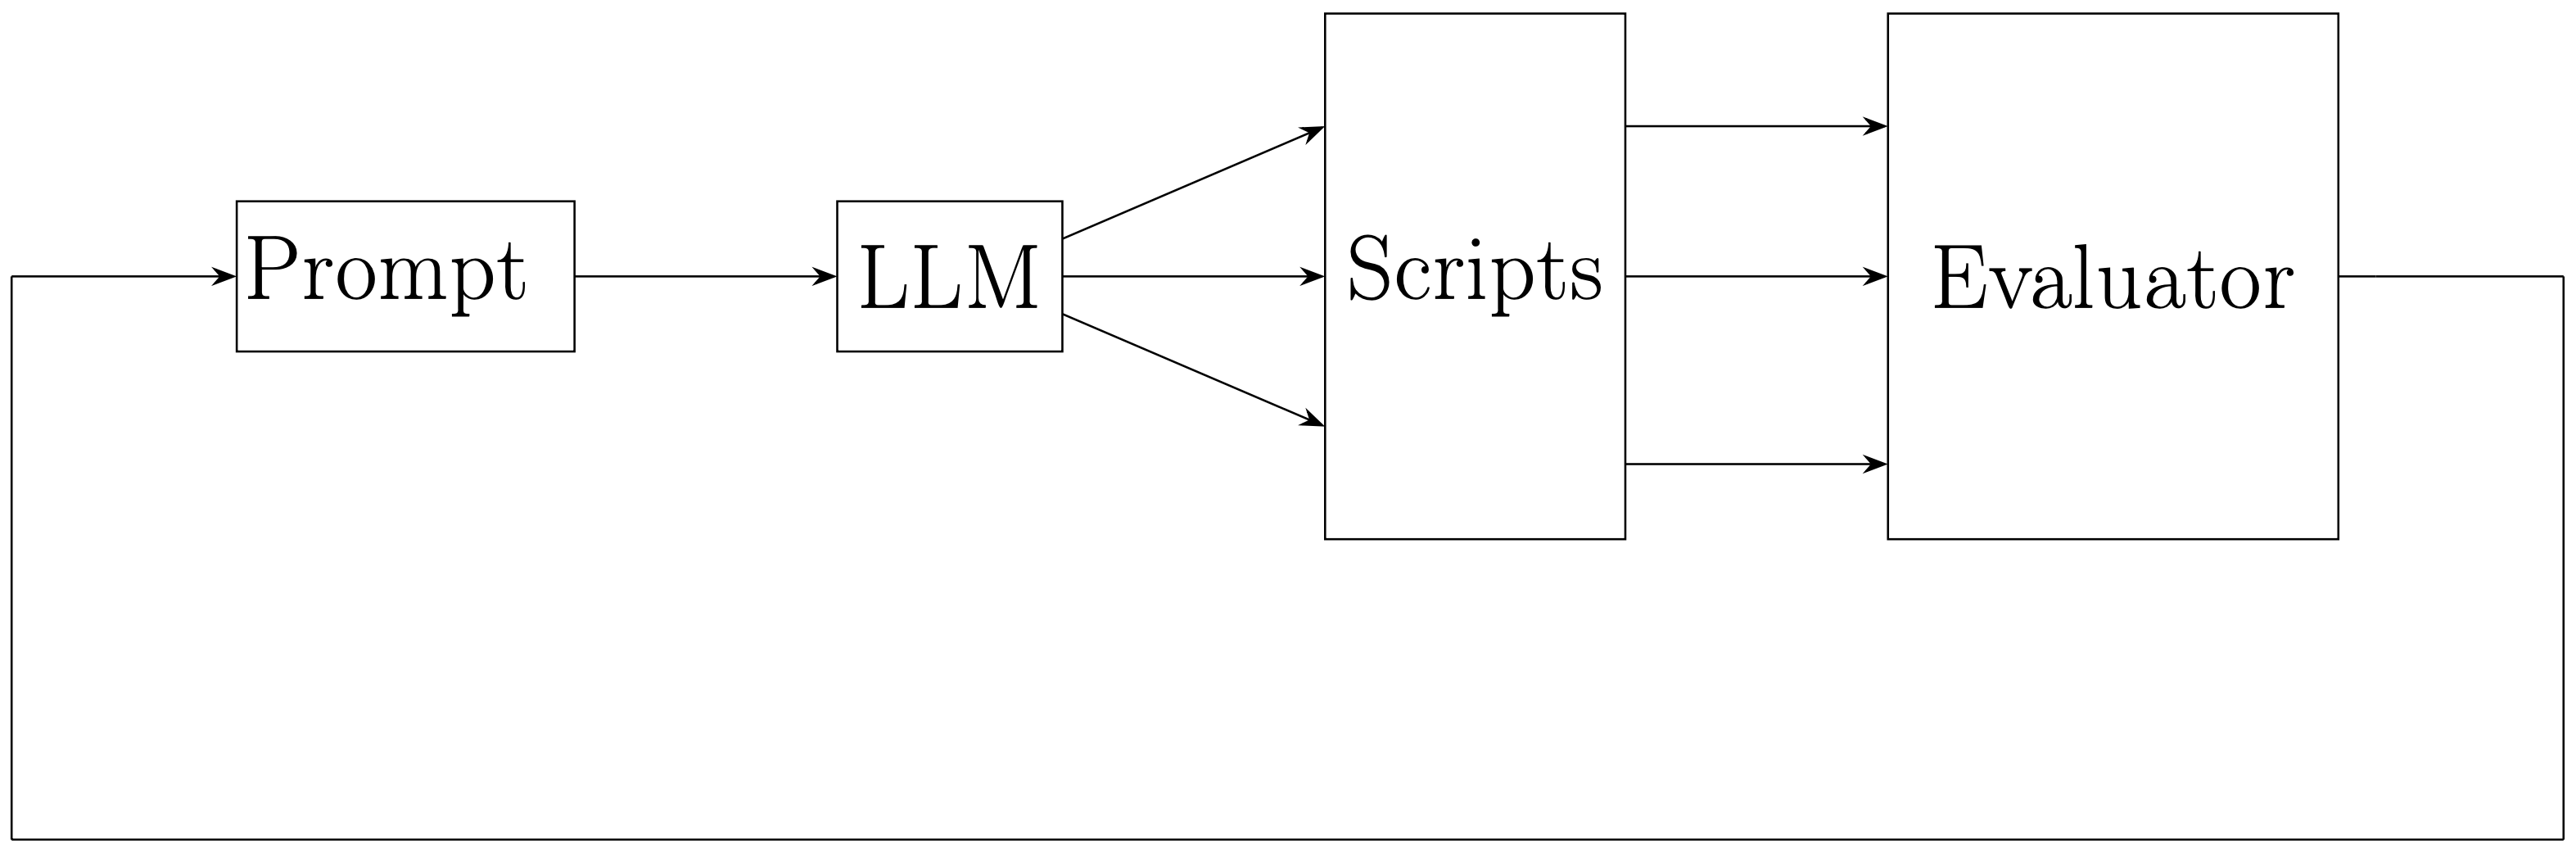
\includegraphics[width=.85\textwidth]{Workflow.png}
  \end{center}
  \begin{flushright}
    \small from \emph{Ellenberg et al.~(2025)}
  \end{flushright}
\end{frame}

%%%%%%%%%%%%%%%%%%%%%%%%%%%%%%%%%%%%%%%%%%%%%%

\begin{frame}
  \frametitle{Four components, one iteration}
  \pause
  \begin{itemize}
    \setlength{\itemsep}{.1cm}
    \item[\textbf{1.}] \bemph{Program database} -- all programs so far,
      ranked by performance + diversity.
      \pause
    \item[\textbf{2.}] \bemph{Prompt sampler} -- picks good + varied programs,
      assembles the prompt.
      \pause
    \item[\textbf{3.}] \bemph{LLM ensemble} -- Gemini Flash (fast / broad)
      + Gemini Pro (slow / deep) write a child program.
      \pause
    \item[\textbf{4.}] \bemph{Evaluator pool} -- runs, scores, returns to
      database if interesting.
  \end{itemize}
  \pause
  \vspace{.25cm}

  Prompt template:
  \emph{``Here are \(k\) programs solving \(P\) with scores
    \(s_1, \ldots, s_k\); write a higher-scoring one.''}
  \pause
  \vspace{.2cm}

  \begin{center}
    Repeat \(\sim 10^6 \) times.
  \end{center}
\end{frame}

%%%%%%%%%%%%%%%%%%%%%%%%%%%%%%%%%%%%%%%%%%%%%%

\begin{frame}
  \frametitle{What is \emph{actually} being evolved?}
  \pause
  Not the mathematical object itself, but the \remph{program that constructs it}.
  \pause
  \vspace{.3cm}

  \begin{itemize}
    \item[$\bullet$] \bemph{Cap set.} Evolve a function that decides which
      vectors to add next.
      \pause
    \item[$\bullet$] \bemph{Ramsey graphs.} Evolve a search algorithm that
      builds large graphs avoiding monochromatic cliques.
      \pause
    \item[$\bullet$] \bemph{Matrix multiplication.} Evolve an entire
      gradient-based solver for low-rank tensor decomposition.
  \end{itemize}
  \pause
  \vspace{.3cm}

  Programs are typically \emph{interpretable} -- humans can read and
  understand them.
\end{frame}

%%%%%%%%%%%%%%%%%%%%%%%%%%%%%%%%%%%%%%%%%%%%%%
%% § 5. Examples
%%%%%%%%%%%%%%%%%%%%%%%%%%%%%%%%%%%%%%%%%%%%%%

\section{Discoveries}

%%%%%%%%%%%%%%%%%%%%%%%%%%%%%%%%%%%%%%%%%%%%%%
%% 5a. Cap set
%%%%%%%%%%%%%%%%%%%%%%%%%%%%%%%%%%%%%%%%%%%%%%

\begin{frame}
  \frametitle{Example 1: the Cap Set problem}
  \begin{prob}[Cap Set]
    Find the largest subset of \( (\ZZ/3\ZZ)^n \) containing no three
    elements \( a, b, c \) with \( a + b + c = 0 \).
  \end{prob}
  \pause
  \vspace{.2cm}

  \begin{itemize}
    \item[$\bullet$] Equivalently: no three vectors on a line (3-term AP). \pause
    \item[$\bullet$] Exact size known only for \( n \le 6 \); search space
      grows like \( 3^n \). \pause
    \item[$\bullet$] Dimension 8: previous record \emph{496}, stood
      $\sim 20$ years.
  \end{itemize}
\end{frame}

%%%%%%%%%%%%%%%%%%%%%%%%%%%%%%%%%%%%%%%%%%%%%%

\begin{frame}
  \frametitle{Example 1: the Cap Set problem}
  \begin{center}
    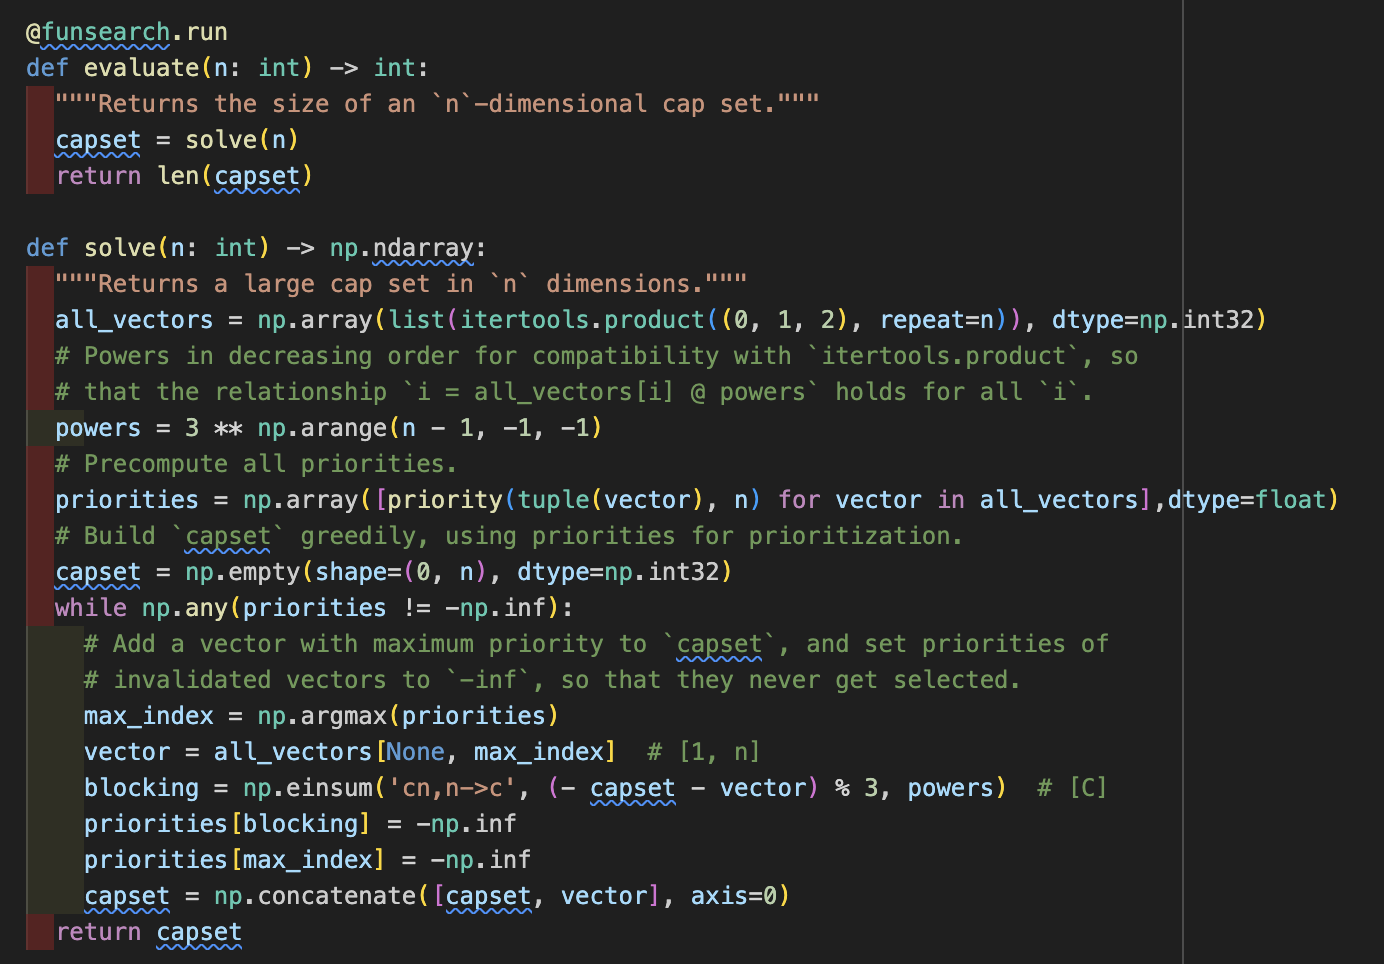
\includegraphics[height=5cm]{FunSearch_Eval_Solve.png}
  \end{center}
  \pause
  FunSearch: cap set of size \remph{512} in dimension 8.
  First improvement in 20 years; the program is \emph{human-readable}.
\end{frame}

%%%%%%%%%%%%%%%%%%%%%%%%%%%%%%%%%%%%%%%%%%%%%%

\begin{frame}[fragile]
  \frametitle{Example 1: the priority function}
  \begin{block}{What FunSearch evolves}
  \scriptsize
  \begin{verbatim}
  def priority(v: tuple[int, ...], n: int) -> float:
    """Returns the priority of vector v.
    The cap set is built by adding vectors that
    do not create a 3-term AP, in order of priority.
    """
    return 0.0
  \end{verbatim}
  \normalsize
  \end{block}
  \pause
  \vspace{.2cm}

  From this trivial seed, FunSearch evolves a heuristic that --
  run greedily -- produces a record cap set.
\end{frame}

%%%%%%%%%%%%%%%%%%%%%%%%%%%%%%%%%%%%%%%%%%%%%%
%% 5b. Ramsey
%%%%%%%%%%%%%%%%%%%%%%%%%%%%%%%%%%%%%%%%%%%%%%

\begin{frame}
  \frametitle{Example 2: Ramsey numbers}
  \begin{prob}[Party problem]
    The smallest \( N \) such that every gathering of \( N \) people
    contains either 3 mutual friends or 3 mutual strangers is
    \( R(3,3) = 6 \).
  \end{prob}
  \pause
  \vspace{.3cm}

  In general, \( R(s,t) \) is the smallest \( N \) such that any 2-coloring
  of the edges of \( K_N \) contains a red \( K_s \) or a blue \( K_t \).
  \pause
  \vspace{.3cm}

  \begin{center}
  \footnotesize
  \begin{tabular}{c|cccc}
    \( s \backslash t \) & 3 & 4 & 5 & 6 \\
    \hline
    3 & 6 & 9 & 14 & 18 \\
    4 &   & 18 & 25 & \( \in [36, 41] \) \\
    5 &   &    & \remph{\( \in [43, 48] \)} & \\
  \end{tabular}
  \end{center}
\end{frame}

%%%%%%%%%%%%%%%%%%%%%%%%%%%%%%%%%%%%%%%%%%%%%%

\begin{frame}
  \frametitle{Example 2: the small-Ramsey table}
  Each entry: \emph{decades} of bespoke human computer searches.
  \pause

  \begin{center}
    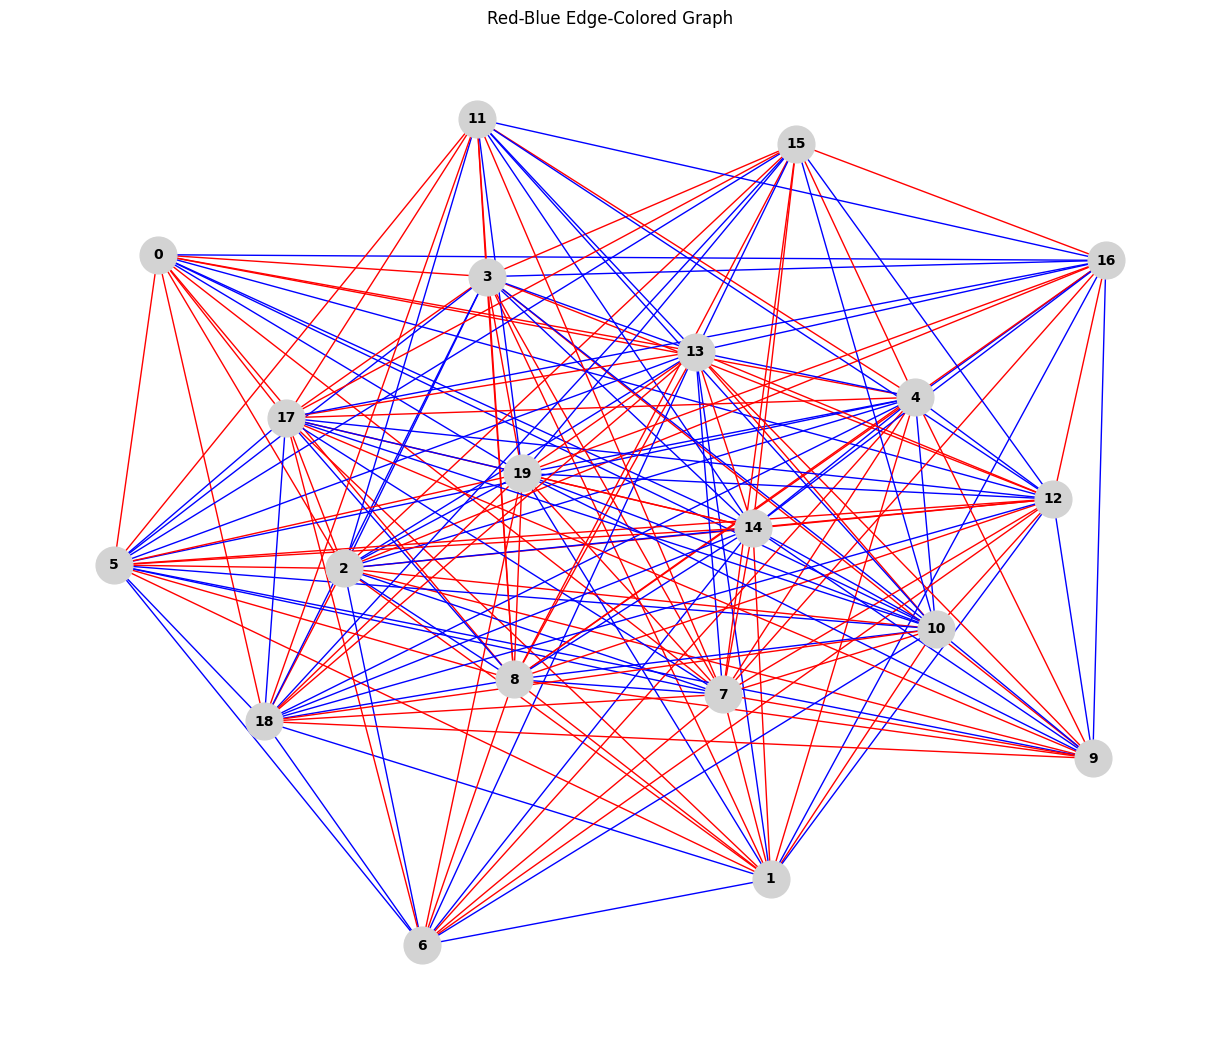
\includegraphics[height=4cm]{r44-14.png}
  \end{center}
  \pause

  Above: 2-coloring of \( K_{14} \), no monochromatic \( K_4 \).
  Witness for \( R(4,4) > 14 \).
\end{frame}

%%%%%%%%%%%%%%%%%%%%%%%%%%%%%%%%%%%%%%%%%%%%%%

\begin{frame}
  \frametitle{Example 2: AlphaEvolve takes a single shot}
  \emph{Nagda et al.}\ (\texttt{arXiv:2603.09172}): AlphaEvolve as a
  \remph{single meta-algorithm} against the Ramsey table.
  \pause
  \vspace{.2cm}

  \begin{center}
    \footnotesize
    \begin{tabular}{l|cc}
      Number & previous & AlphaEvolve \\
      \hline
      \( R(3,13) \) & 60 & \remph{61} \\
      \( R(3,18) \) & 99 & \remph{100} \\
      \( R(4,13) \) & 138 & \remph{139} \\
      \( R(4,14) \) & 147 & \remph{148} \\
      \( R(4,15) \) & 158 & \remph{159} \\
      \( R(4,16) \) & 170 & \remph{174} \\
      \( R(4,18) \) & 205 & \remph{209} \\
      \( R(4,19) \) & 213 & \remph{219} \\
      \( R(4,20) \) & 234 & \remph{237} \\
    \end{tabular}
  \end{center}
  \pause
  \vspace{.2cm}

  \emph{One} system improved \emph{nine} classical lower bounds.
\end{frame}

%%%%%%%%%%%%%%%%%%%%%%%%%%%%%%%%%%%%%%%%%%%%%%
%% 5c. Matrix multiplication --- HOOK RECOVERY
%%%%%%%%%%%%%%%%%%%%%%%%%%%%%%%%%%%%%%%%%%%%%%

\begin{frame}
  \frametitle{Example 3: remember the 49?}
  \pause
  \begin{center}
    \large
    Two \( 4 \times 4 \) matrices: \\
    \pause
    \vspace{.3cm}
    Strassen \( \times \) Strassen: \remph{49} multiplications. \\
    \pause
    \vspace{.4cm}
    AlphaEvolve, May 2025: \remph{48} multiplications.
    \pause
    \vspace{.6cm}

    \normalsize
    First improvement over Strassen \emph{after 56 years}, over any
    field of characteristic 0.
  \end{center}
\end{frame}

%%%%%%%%%%%%%%%%%%%%%%%%%%%%%%%%%%%%%%%%%%%%%%

\begin{frame}
  \frametitle{Example 3: how was it found?}
  Input: a generic gradient-based solver for low-rank tensor decomposition
  (same problem class as Strassen).
  \pause
  \vspace{.3cm}

  \begin{itemize}
    \item[$\bullet$] \bemph{What evolves:} the solver's \emph{code} --
      initializer, loss, optimizer.
      \pause
    \item[$\bullet$] \bemph{Evaluator:} run on the \( 4 \times 4 \) matmul
      tensor; return the rank achieved.
      \pause
    \item[$\bullet$] \bemph{Trick discovered:} \emph{complex} coefficients
      with magic cancellations.
  \end{itemize}
  \pause
  \vspace{.3cm}

  Also: state of the art for \( 13 \) other matmul targets.
\end{frame}

%%%%%%%%%%%%%%%%%%%%%%%%%%%%%%%%%%%%%%%%%%%%%%

\begin{frame}
  \frametitle{Beyond \( 4 \times 4 \): AlphaEvolve in Google's compute stack}
  Same agent, four \emph{separate} engineering problems.
  \pause
  \vspace{.3cm}

  \begin{itemize}
    \item[$\bullet$] Evolved matmul kernel: \remph{\( 23\% \) faster} on
      Gemini training hardware. $\sim 1\%$ of total training time saved.
      \pause
    \item[$\bullet$] Evolved scheduler: recovers \remph{\( 0.7\% \)} of
      Google's worldwide compute.
      \pause
    \item[$\bullet$] Evolved register-allocation hint: \remph{\( 32\% \)}
      shorter FlashAttention runtime.
  \end{itemize}
  \pause
  \vspace{.3cm}

  Pure mathematics and industrial impact, from one system.
\end{frame}

%%%%%%%%%%%%%%%%%%%%%%%%%%%%%%%%%%%%%%%%%%%%%%
%% 4d. Kakeya problem (climax) --- Tao et al.
%%%%%%%%%%%%%%%%%%%%%%%%%%%%%%%%%%%%%%%%%%%%%%

\begin{frame}
  \frametitle{Example 4: the Kakeya needle problem}
  \begin{prob}[Kakeya, 1917]
    Can a unit needle be rotated in the plane while sweeping out an
    \remph{arbitrarily small} area?
  \end{prob}
  \pause
  \vspace{.1cm}

  \begin{center}
    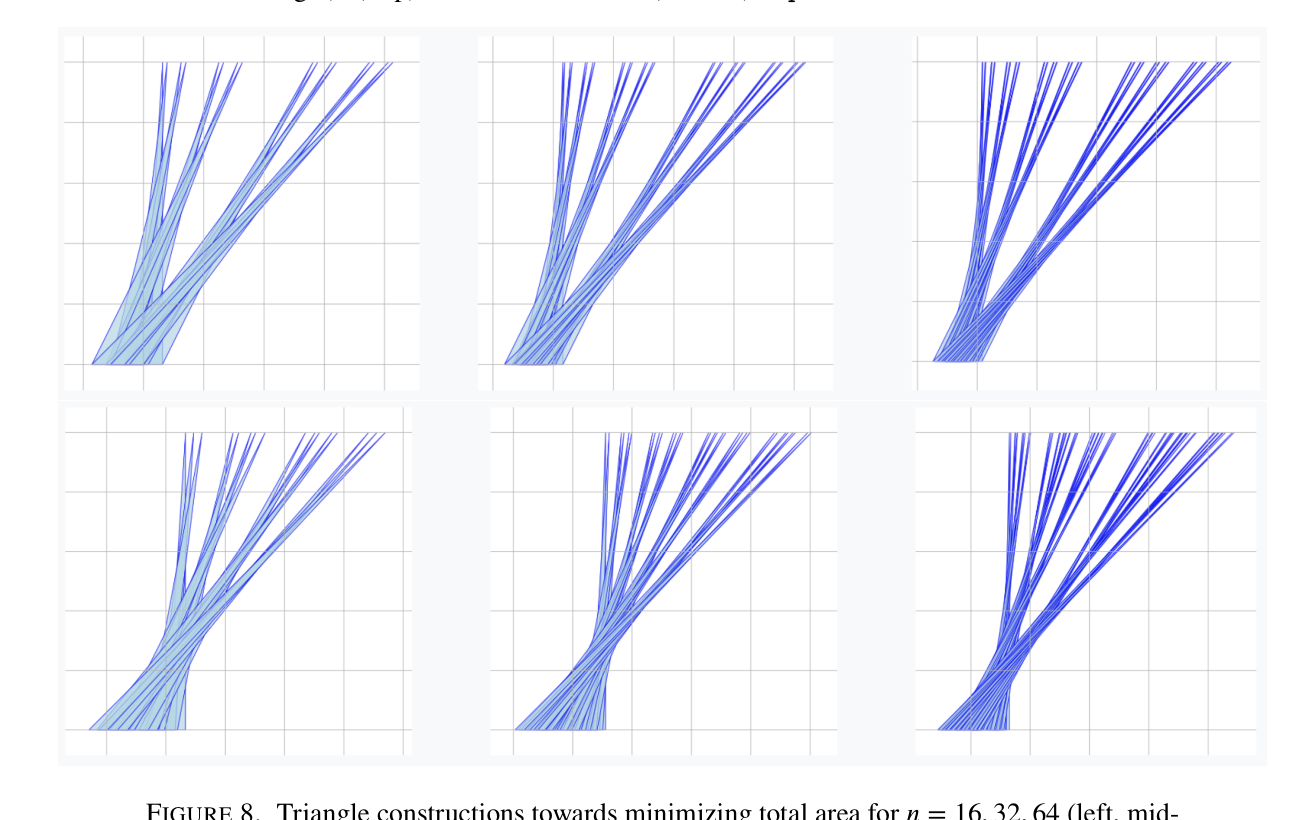
\includegraphics[height=3.4cm]{kakeya_needle_2D_triangle.png}
  \end{center}
  \pause
  \vspace{-.05cm}

  \begin{itemize}
    \setlength{\itemsep}{.05cm}
    \item[$\bullet$] Yes (Besicovitch, 1928): \emph{measure-zero} sets exist.
    \item[$\bullet$] \bemph{Kakeya set}: contains a unit segment in every direction.
    \item[$\bullet$] \bemph{Kakeya conjecture}: \( \dim_H(K) = d \) in \( \RR^d \).
      \quad (3D: Wang--Zahl, 2025.)
  \end{itemize}
\end{frame}

%%%%%%%%%%%%%%%%%%%%%%%%%%%%%%%%%%%%%%%%%%%%%%

\begin{frame}
  \frametitle{Example 4: from \(\RR^d\) to \(\FF_q^d\)}
  Same combinatorics, finite stage.
  \pause
  \vspace{.2cm}

  \begin{prob}[finite field Kakeya]
    Let \( \FF_q \) be a finite field, \( d \ge 1 \). A \bemph{Kakeya set}
    \( K \subseteq \FF_q^d \) contains an entire \emph{line} in every
    direction. \\
    Let \( C^K(d, q) \) be the minimum size of \( K \).
  \end{prob}
  \pause
  \vspace{.1cm}

  \begin{itemize}
    \setlength{\itemsep}{.1cm}
    \item[$\bullet$] \bemph{Dvir (2008)}, polynomial method:
      \( C^K(d, q) \ge c_d \, q^d \).
    \pause
    \item[$\bullet$] Best known upper bound (Bukh--Chao):
      \[
        C^K(d, q) \;\le\; \frac{1}{2^{d-1}}\, q^d + O(q^{d-1}).
      \]
    \pause
    \item[$\bullet$] \emph{Open}: exact constants and \remph{lower-order} terms.
  \end{itemize}
\end{frame}

%%%%%%%%%%%%%%%%%%%%%%%%%%%%%%%%%%%%%%%%%%%%%%

\begin{frame}
  \frametitle{Example 4: a generalizer, not just a finder}
  Two ways to use such a system:
  \pause
  \vspace{.2cm}

  \begin{itemize}
    \setlength{\itemsep}{.15cm}
    \item[$\bullet$] \bemph{Search mode} -- evolve a heuristic that finds
      the best object for a single \( q \).
    \pause
    \item[$\bullet$] \bemph{Generalizer mode} -- evolve a Python function
      that, \emph{given any prime \( p \)}, outputs an explicit Kakeya set.
  \end{itemize}
  \pause
  \vspace{.2cm}

  \begin{KeyIdea}
    Score = \emph{average} normalized size across \emph{many} primes \( p \). \\
    The same code must work simultaneously for all of them. \\
    \(\Rightarrow\) Surviving code \remph{must} be a formula in \( p \).
  \end{KeyIdea}
  \pause
  \vspace{.2cm}

  \begin{center}
    Output: a \remph{closed-form formula} -- not a numerical optimum.
  \end{center}
\end{frame}

%%%%%%%%%%%%%%%%%%%%%%%%%%%%%%%%%%%%%%%%%%%%%%

\begin{frame}
  \frametitle{Example 4: the discovery (\(d = 3\))}
  \begin{AlphaEvolveResult}
    For every prime \( p \equiv 1 \pmod{4} \),
    \[
      C^K(3, p) \;\le\; \tfrac{1}{4} p^3 + \tfrac{7}{8} p^2 - \tfrac{1}{8}.
    \]
  \end{AlphaEvolveResult}
  \pause
  \vspace{.1cm}

  Explicit construction
  (\( g = \tfrac{p-1}{4},\ S = \) quadratic residues in \( \FF_p \)):
  \[
    \Big\{ \big(x,\ \tfrac{q_1+q_2}{2} - x^2 - g,\ \tfrac{q_1-q_2}{2}\big)
      : x \in \FF_p,\ q_1, q_2 \in S \Big\} \;\cup\; \cdots
  \]
  \pause
  \vspace{.1cm}

  \begin{itemize}
    \item[$\bullet$] Bukh--Chao baseline:
      \( \tfrac{1}{4} p^3 + \tfrac{7}{8} p^2 + \textcolor{red}{O(p)} \).
    \pause
    \item[$\bullet$] AlphaEvolve: \emph{exact} cubic and quadratic coefficients,
      \remph{exact} lower-order term \( -\tfrac{1}{8} \).
  \end{itemize}
\end{frame}

%%%%%%%%%%%%%%%%%%%%%%%%%%%%%%%%%%%%%%%%%%%%%%

\begin{frame}
  \frametitle{Example 4: from pattern to formal proof}
  AlphaEvolve discovers; \emph{but who proves the formula?}
  \pause
  \vspace{.15cm}

  \begin{center}
    \begin{tikzpicture}[
      >={Latex[length=2.5mm]},
      node distance=0.5cm and 0.4cm,
      every node/.append style={font=\footnotesize},
      box/.style={rectangle, rounded corners=2pt, draw, semithick,
                  minimum height=1.0cm, minimum width=2.7cm, align=center,
                  fill=white},
      mbox/.style={box, fill=blue!12},
      hbox/.style={box, fill=red!12},
    ]
      \node[hbox] (AE) {\remph{AlphaEvolve} \\ \scriptsize discovers code};
      \node[mbox, right=of AE] (DT) {\bemph{Deep Think} \\ \scriptsize natural-language proof};
      \node[mbox, right=of DT] (AP) {\bemph{AlphaProof} \\ \scriptsize Lean formal proof};
      \draw[->,semithick] (AE) -- (DT);
      \draw[->,semithick] (DT) -- (AP);
    \end{tikzpicture}
  \end{center}
  \pause
  \vspace{.1cm}

  \begin{itemize}
    \setlength{\itemsep}{.05cm}
    \item[$\bullet$] \( d = 3 \): \remph{all three steps automated}.
      Proof uses only \texttt{mathlib} number theory.
    \pause
    \item[$\bullet$] \( d = 4 \): Deep Think reveals \emph{elliptic curves};
      AlphaProof gives up. Humans verify by hand.
    \pause
    \item[$\bullet$] \( d = 5 \):
      \( \tfrac{1}{16} p^5 + \tfrac{47}{128} p^4 + \tfrac{177}{256} p^3 + O(p^{5/2}) \),
      verified by hand.
  \end{itemize}
\end{frame}

%%%%%%%%%%%%%%%%%%%%%%%%%%%%%%%%%%%%%%%%%%%%%%

\begin{frame}
  \frametitle{Example 4: from AI to new theorems}
  Two follow-up papers \emph{by Tao alone}, both inspired by AlphaEvolve:
  \pause
  \vspace{.15cm}

  \begin{itemize}
    \setlength{\itemsep}{.1cm}
    \item[$\bullet$] \bemph{Nikodym sets} -- AlphaEvolve's complicated first
      try \(\to\) human simplification \(\to\) new asymptotic
      \[
        C^N(d, p) \;\le\; p^d - \big( \tfrac{d-2}{\log 2} + 1 + o(1) \big)\, p^{d-1} \log p.
      \]
    \pause
    \item[$\bullet$] \bemph{Arithmetic Kakeya}: AlphaEvolve's distributions
      resemble \emph{discrete Gaussians}:
  \end{itemize}
  \begin{center}
    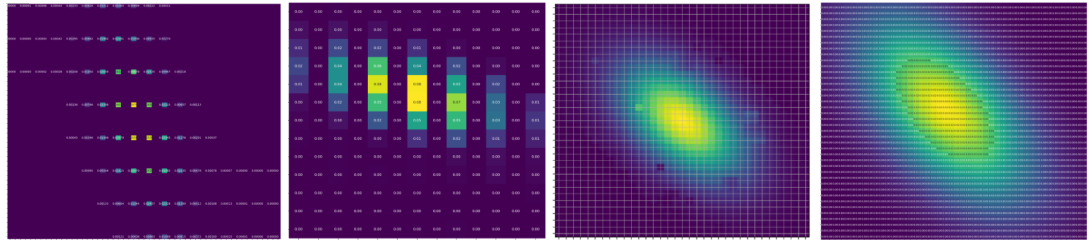
\includegraphics[height=1.9cm]{arithmetic_kakeya_distributions.png}
  \end{center}
  \pause
  \vspace{-.1cm}

  \(\to\) New theorem of Tao:
  \(
    C\big(\{0,1,\infty\}; \tfrac{a}{b}\big)
    = 2 - \Theta\big(\tfrac{1}{\log(2 + |a| + |b|)}\big).
  \)
  \pause
  \vspace{.05cm}

  \begin{center}
    \emph{AI suggested the pattern. The mathematicians proved the theorem.}
  \end{center}
\end{frame}

%%%%%%%%%%%%%%%%%%%%%%%%%%%%%%%%%%%%%%%%%%%%%%
%% § 6. Limitations
%%%%%%%%%%%%%%%%%%%%%%%%%%%%%%%%%%%%%%%%%%%%%%

\section{Limitation and message}

%%%%%%%%%%%%%%%%%%%%%%%%%%%%%%%%%%%%%%%%%%%%%%

\begin{frame}
  \frametitle{What AlphaEvolve cannot (yet) do}
  \pause
  \begin{itemize}
    \item[$\bullet$] \bemph{No proofs.} Constructions and heuristics, not
      theorems. (Tao Kakeya: Deep Think + AlphaProof close the gap.)
      \pause
      \vspace{.2cm}
    \item[$\bullet$] \bemph{Needs an evaluator.} No automatic score
      \(\Rightarrow\) nothing to evolve.
      \pause
      \vspace{.2cm}
    \item[$\bullet$] \bemph{Bijections are hard.} (\texttt{arXiv:2511.20987}:
      These agents struggle with combinatorial bijections.)
      \pause
      \vspace{.2cm}
    \item[$\bullet$] \bemph{Compute cost.} Nontrivial runs: need costs for LLM API calls.
  \end{itemize}
\end{frame}

%%%%%%%%%%%%%%%%%%%%%%%%%%%%%%%%%%%%%%%%%%%%%%

\begin{frame}
  \frametitle{The message}
  \pause
  \begin{center}
    \large
    AlphaEvolve does \remph{not} replace mathematicians. \\
    \pause
    \vspace{.4cm}
    It is a new \bemph{collaborator} in the loop.
  \end{center}
  \pause
  \vspace{.5cm}

  Tao's finite-field Kakeya -- the prototype:
  \begin{itemize}
    \item[$\bullet$] AI: closed-form Kakeya sets, all primes at once.
      \pause
    \item[$\bullet$] Humans: spotted the structure, formalized the proof,
      proved new theorems.
  \end{itemize}
\end{frame}

%%%%%%%%%%%%%%%%%%%%%%%%%%%%%%%%%%%%%%%%%%%%%%
%% § 7. Try it yourself
%%%%%%%%%%%%%%%%%%%%%%%%%%%%%%%%%%%%%%%%%%%%%%

\section{Try it yourself}

%%%%%%%%%%%%%%%%%%%%%%%%%%%%%%%%%%%%%%%%%%%%%%

\begin{frame}
  \frametitle{The Evolve ecosystem}
  AlphaEvolve runs \emph{only} inside DeepMind --
  but the paradigm has gone open.
  \pause
  \vspace{.2cm}

  \begin{itemize}
    \setlength{\itemsep}{.15cm}
    \item[$\bullet$] \bemph{Ellenberg et al.} (\texttt{arXiv:2503.11061}) --
      FunSearch \bemph{for working mathematicians}: any commercial LLM API,
      no HPC, one Python file (\emph{priority} + \emph{evaluator}).
    \item[$\bullet$] \bemph{OpenEvolve} -- community open-source clone
      (\texttt{github.com/algorithmicsuperintelligence/openevolve}).
    \pause
    \item[$\bullet$] \bemph{ShinkaEvolve} (\texttt{arXiv:2509.19349}, ICLR 2026) --
      Sakana AI; sample-efficient. New 26-circle packing SOTA with only
      150 LLM samples.
    \pause
    % \item[$\bullet$] \bemph{FlowBoost} (\texttt{arXiv:2601.18005}, 2026) --
    %   LLM-free alternative (flow matching). Beats AlphaEvolve on some
    %   packing problems.
    % \pause
  \end{itemize}
  \pause
  \vspace{.2cm}

  \begin{center}
    A tool you can run \remph{on a laptop, today}.
  \end{center}
\end{frame}

%%%%%%%%%%%%%%%%%%%%%%%%%%%%%%%%%%%%%%%%%%%%%%

\begin{frame}
  \frametitle{Two starter problems}
  \begin{prob}[Recover a known Ramsey bound]
    Re-discover a 2-coloring of \( K_{17} \) with no monochromatic
    \( K_4 \) (so that \( R(4,4) \ge 18 \)).
    \\ \pause
    \emph{Evaluator:} count monochromatic \( K_4 \)'s in a candidate
    coloring; reward \( = -\#\text{monochromatic } K_4 \).
  \end{prob}
  \pause
  \vspace{.3cm}

  \begin{prob}[No-isosceles subset of a small grid]
    In an \( n \times n \) grid, find as many points as possible such
    that no three of them form an isosceles triangle.
    \\ \pause
    \emph{Evaluator:} for each triple, check the three pairwise distances.
  \end{prob}
\end{frame}

%%%%%%%%%%%%%%%%%%%%%%%%%%%%%%%%%%%%%%%%%%%%%%

\begin{frame}
  \frametitle{Designing your own problem}
  Ready for an evolutionary coding agent when:
  \pause
  \vspace{.3cm}

  \begin{itemize}
    \item[\textbf{1.}] Candidates expressible as Python code.
      \pause
      \vspace{.2cm}
    \item[\textbf{2.}] A \remph{deterministic} evaluator returns a
      real-valued score in seconds (or less).
      \pause
      \vspace{.2cm}
    \item[\textbf{3.}] Meaningful gap from trivial baseline to SOTA --
      somewhere to climb.
  \end{itemize}
\end{frame}

%%%%%%%%%%%%%%%%%%%%%%%%%%%%%%%%%%%%%%%%%%%%%%

% \begin{frame}
%   \frametitle{What should we teach our students?}
%   \pause
%   \begin{itemize}
%     \item[$\bullet$] \bemph{Mathematical literacy:} formulating problems
%       so a machine can score candidates -- a \emph{deeply mathematical} skill.
%       \pause
%       \vspace{.2cm}
%     \item[$\bullet$] \bemph{Programming as scratch paper:} coding lets
%       students \emph{ask their own questions}.
%       \pause
%       \vspace{.2cm}
%     \item[$\bullet$] \bemph{Verification, not authority:} ``is this correct?''
%       \(\to\) \emph{run the evaluator}, don't \emph{trust the LLM}.
%   \end{itemize}
% \end{frame}

%%%%%%%%%%%%%%%%%%%%%%%%%%%%%%%%%%%%%%%%%%%%%%

\begin{frame}
  \frametitle{Three takeaways}
  \pause
  \begin{enumerate}[label=\textbf{\arabic*.}]
    \item AI can now \remph{discover} new mathematics --
      not just compute or verify.
      \pause
      \vspace{.3cm}
    \item Trust comes from the \remph{evaluator}, not the LLM.
      \pause
      \vspace{.3cm}
    \item The model is \remph{collaboration} -- AI generates patterns;
      humans recognize structure and prove theorems.
  \end{enumerate}
\end{frame}

%%%%%%%%%%%%%%%%%%%%%%%%%%%%%%%%%%%%%%%%%%%%%%

\begin{frame}
  \begin{center}
    \Huge Thank you!
  \end{center}
\end{frame}

%%%%%%%%%%%%%%%%%%%%%%%%%%%%%%%%%%%%%%%%%%%%%%
%% Backup: References + Bruhat supplementary
%%%%%%%%%%%%%%%%%%%%%%%%%%%%%%%%%%%%%%%%%%%%%%

\appendix

% Backup: hide footer + exclude from main frame count
\setbeamertemplate{footline}{}

\section*{}

\begin{frame}[noframenumbering]
  \frametitle{References (key papers)}
  \footnotesize
  \begin{itemize}
    \item[$\bullet$] Romera-Paredes et al., \emph{Mathematical discoveries from program search with large language models}, Nature 625 (2024) 468--475. \quad [FunSearch]
    \item[$\bullet$] Novikov et al., \emph{AlphaEvolve: A coding agent for scientific and algorithmic discovery}, \texttt{arXiv:2506.13131} (2025).
    \item[$\bullet$] Ellenberg, Fraser-Taliente, Harvey, Srivastava, Sutherland, \emph{Generative modeling for mathematical discovery}, \texttt{arXiv:2503.11061} (2025).
    \item[$\bullet$] Georgiev, G\'omez-Serrano, Tao, Wagner, \emph{Mathematical exploration and discovery at scale}, \texttt{arXiv:2511.02864} (2025).
    \item[$\bullet$] Ellenberg, Libedinsky, Plaza, Simental, Williamson, \emph{Bruhat intervals that are large hypercubes}, \texttt{arXiv:2601.01235} (2026).
    \item[$\bullet$] Nagda, Raghavan, Thakurta, \emph{Reinforced generation of combinatorial structures: Ramsey numbers}, \texttt{arXiv:2603.09172} (2026).
  \end{itemize}
\end{frame}

%%%%%%%%%%%%%%%%%%%%%%%%%%%%%%%%%%%%%%%%%%%%%%

\section*{Supplementary}

\begin{frame}[noframenumbering]
  \frametitle{Supplement: hypercubes inside Bruhat order}
  The symmetric group \( S_n \) carries the \bemph{Bruhat order} --
  central in representation theory and flag variety geometry.
  \pause
  \vspace{.2cm}

  \begin{center}
    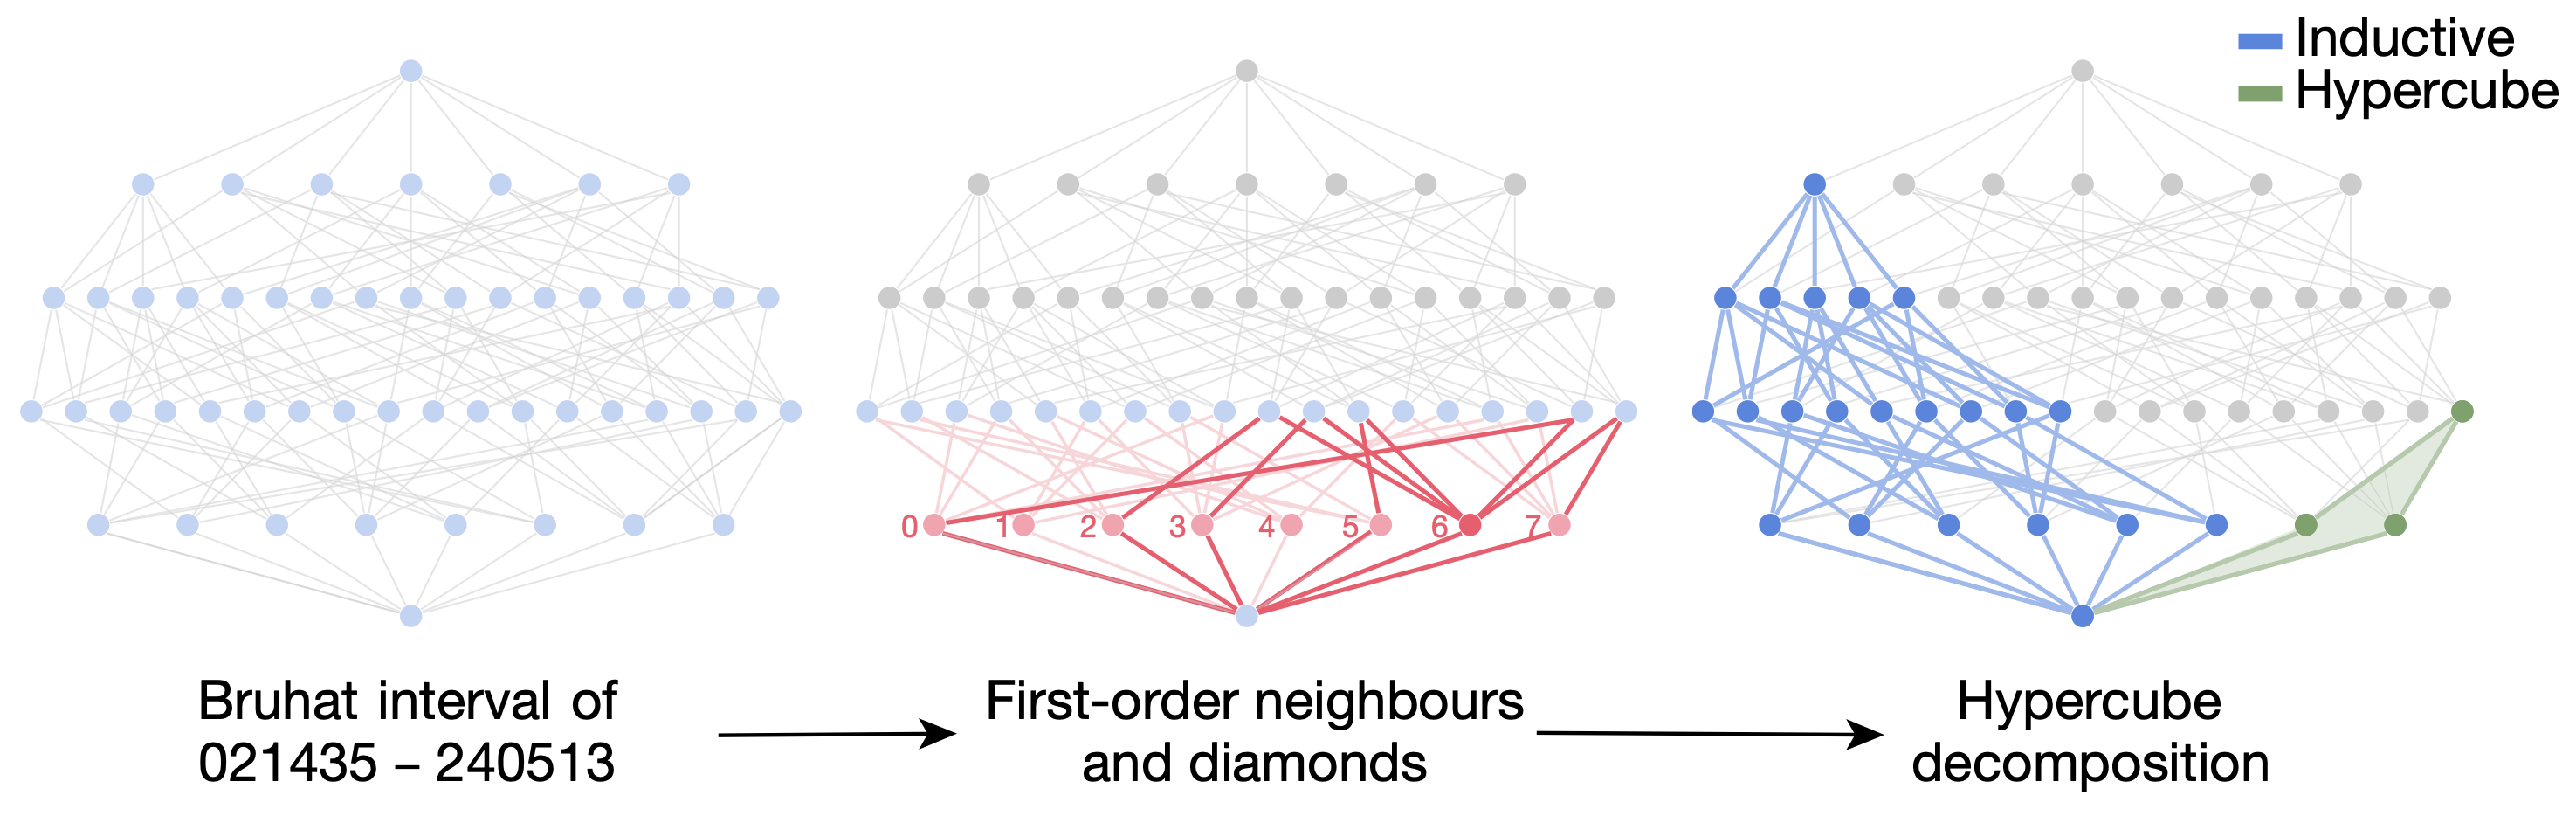
\includegraphics[height=3.2cm]{hypercube.png}
  \end{center}
  \pause
  \vspace{.1cm}

  Goal: large \emph{boolean intervals} (poset hypercubes) in \( S_n \).
  Size controls Kazhdan--Lusztig polynomial coefficients,
  cluster algebra frozen variables, \ldots
\end{frame}

%%%%%%%%%%%%%%%%%%%%%%%%%%%%%%%%%%%%%%%%%%%%%%

\begin{frame}[noframenumbering]
  \frametitle{Supplement: the AlphaEvolve experiment}
  Williamson et al.\ (2026): asked AlphaEvolve for a large hypercube
  interval in \( S_n \).
  \pause
  \vspace{.3cm}

  AlphaEvolve returned a \emph{recipe} (depending on \( n \)),
  excellent for small \( n \).
  \pause
  \vspace{.3cm}

  Surprise: the authors recognized the recipe.
  \pause
  \vspace{.2cm}

  \begin{center}
    The permutations AlphaEvolve picked were exactly the\\
    \remph{dyadically well-distributed} permutations
  \end{center}
  -- a number-theoretic notion from Monte Carlo integration
  and mathematical finance.
\end{frame}

%%%%%%%%%%%%%%%%%%%%%%%%%%%%%%%%%%%%%%%%%%%%%%

\begin{frame}[noframenumbering]
  \frametitle{Supplement: a theorem from the loop}
  \begin{WilliamsonResult}
    For every \( m \ge 1 \), the set of dyadically well-distributed
    permutations in \( S_{2^m} \) forms a Bruhat interval, and that
    interval is poset isomorphic to a hypercube of dimension
    \( m \cdot 2^{m-1} \).
  \end{WilliamsonResult}
  \pause
  \vspace{.3cm}

  Stirling: no Bruhat hypercube in \( S_{2^m} \) exceeds dimension
  \( m \cdot 2^m \). The construction is optimal \emph{up to a factor of 2}.
  \pause
  \vspace{.3cm}

  \begin{center}
    \emph{AI suggested the pattern. The mathematicians proved the theorem.}
  \end{center}
\end{frame}

\end{document}
